\begin{atiTask}[
  title = Gradient und Rotation
  %call = Zusatzaufgabe,
]

Gegeben seien das skalare Vektorfeld
\[
\vec{A}(x,y,z)=xy\vec{i}-y^2z\vec{j}+xz^2\vec{k}
\]
und das skalare Feld
\[
U(x,y,z)=2xyz^2.
\]
Berechnen Sie in kartesischen Koordinaten
\begin{multicols}{2}
\begin{atiSubequations}
\item{\gradient U}
\item{\curl \vec{A}}
\item{\curl (U\vec{A})}
\item{\curl \curl\vec{A}}
\item{\gradient(\vec{A}\cdot \curl\vec{A})}
\item{\curl\gradient U.}
\end{atiSubequations}
\end{multicols}

\end{atiTask}

\begin{atiSolution}
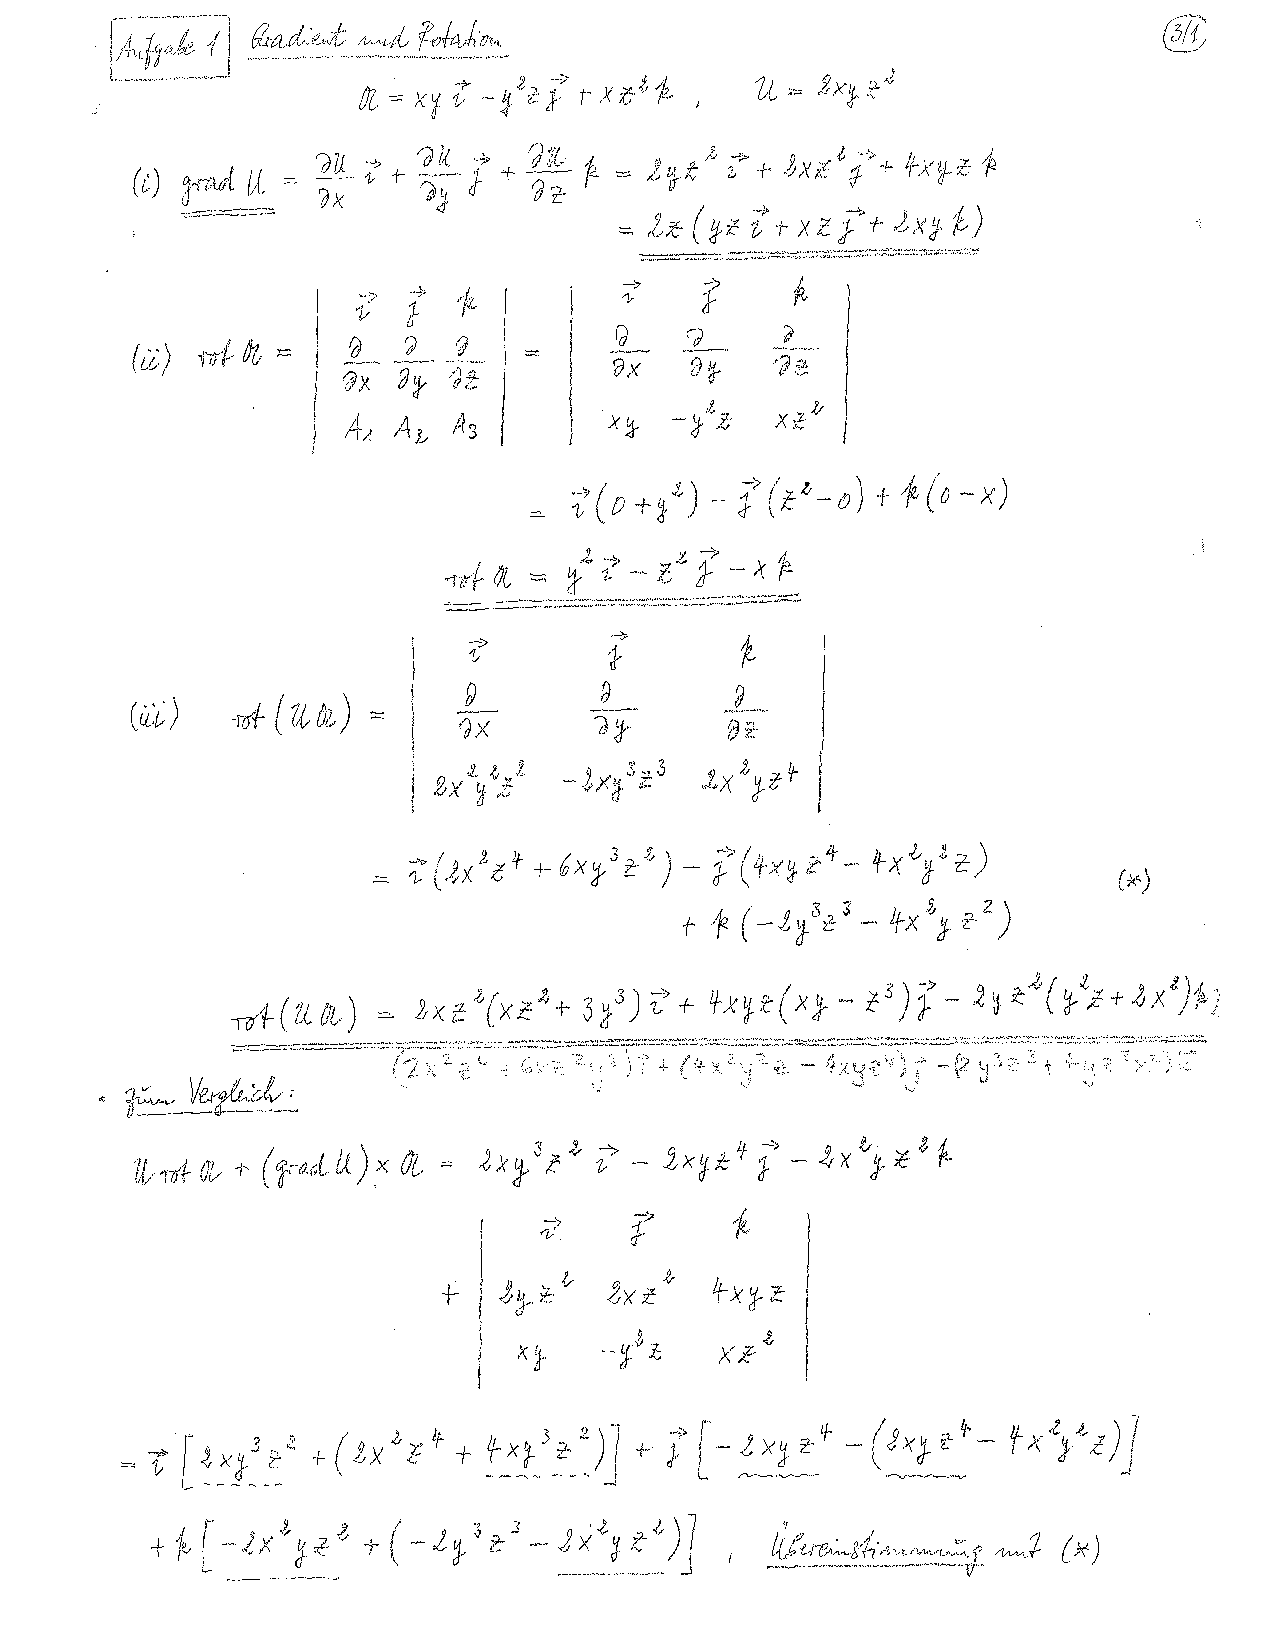
\includepdf{solution-rotation_ii.pdf}
\end{atiSolution}